\section{Dettagli implementativi}\label{sec:implementazione}
In questo paragrafo verranno descritti in modo specifico i dettagli implementativi di ogni modello e di ogni sua versione, oltre ai vari passaggi di pre-processing e il metodo di valutazione.

\subsection{Pre-processing}\label{subsec:prepr}
Per le versioni 1 dei modelli i dati non vengono pre-processati, infatti i dati non vengono modificati come descritto nella sezione \ref{sec:analisi}, ma vengono solamente fatte le modifiche in fase di EDA, modificando quindi i tipi dei dati ed eliminando i valori NaN. Lo splitting in questo caso è fatto quindi sui dati originali, togliendo dalle features lo \textit{user}, che è il nome del soggetto e non influisce sull'apprendimento, ed è stata tolta anche la feature \textit{gender}, in quanto non ancora trasformata con l'encoder. Inoltre la variabile target \textit{class} in questo caso rimane sotto forma di stringa.

Per le versioni 2 invece vengono effettuati gli step di pre-processing descritti brevemente nella sezione \ref{sec:analisi}, in particolare dopo aver fatto l'encoding della feature \textit{gender} e del target \textit{class}, è stata studiata la matrice di correlazione, mostrata in figura \ref{fig:corr}, per valutare la collinearità delle features tra di loro, e con la variabile target. Ne risulta che le variabili \textit{y1} e \textit{y4} sono particolarmente correlate con la variabile target, quindi saranno importanti ai fini della classificazione. In secondo luogo è possibile notare che le features \textit{how\_tall\_in\_meters}, \textit{weight} e \textit{body\_mass\_index} sono particolarmente correlate tra di loro e di conseguenza è conveniente eliminarne due e mantenerne una sola. Infine le tre variabili che rappresentano le coordinate dell'accelerometro 2, quello sulla coscia sinistra, sono molto correlate tra loro, quindi anche in questo caso conviene mantenerne una sola.

\begin{figure}[ht]
    \centering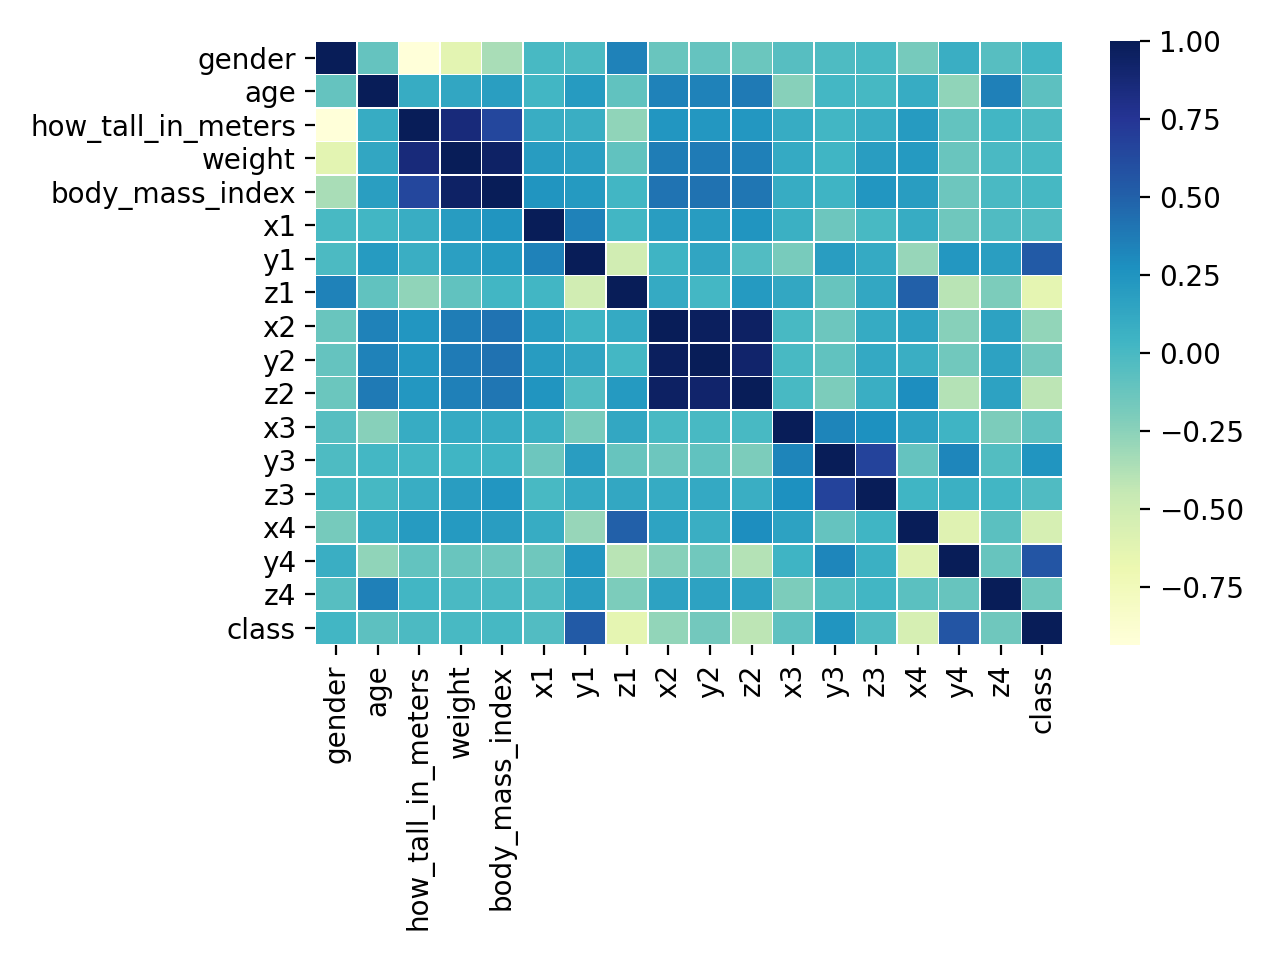
\includegraphics[width=1.0\linewidth]{corr}
    \caption{Matrice di correlazione.}
    \label{fig:corr}
\end{figure}

Dalle informazioni raccolte dalla matrice di correlazione, in figura \ref{fig:corr}, effettuiamo la features selection eliminando le variabili \textit{weight} e \textit{body\_mass\_index} perché altamente correlate con \textit{how\_tall\_in\_meters} e viene mantenuta quest'ultima; vengono anche eliminate le coordinate x e z del secondo accelerometro, mantenendo solo la coordinata y. Infine vengono eliminate le variabili \textit{user} e \textit{age} in quanto non influenti sul riconoscimento della postura.

Le features selezionate vengono poi sottoposte a uno scaling, in particolare si applica il metodo del \textbf{min-max-scaling}: trasforma il valore di ogni features portandolo a un valore compreso tra 0 e 1, per farlo applica a ogni variabile la seguente formula:

\begin{equation}
x' = \frac{x-min(x)}{max(x)-min(x)}
\end{equation}

È importante sottolineare che i parametri $min(x)$ e $max(x)$ vanno calcolati sulla base del solo training set, dopodiché si applica la trasformazione al training set e al test set.

\begin{figure}[ht]
    \centering
    \begin{subfigure}[t]{0.4\textwidth}
        \centering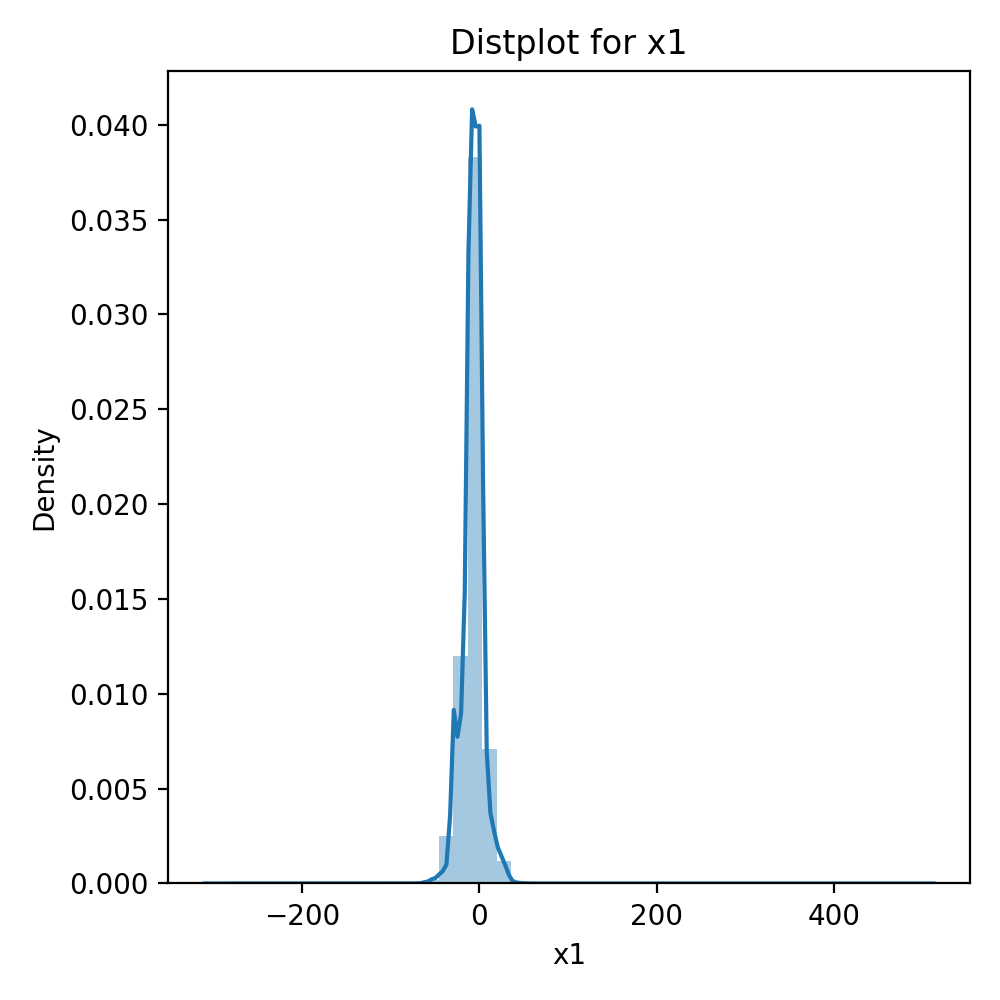
\includegraphics[width=1\linewidth]{x1prescaling}
        \caption{Distribuzione di x1 prima del min-max-scaling.}
        \label{fig:distprescaling:x1}
    \end{subfigure}
    %
    \begin{subfigure}[t]{0.4\textwidth}
        \centering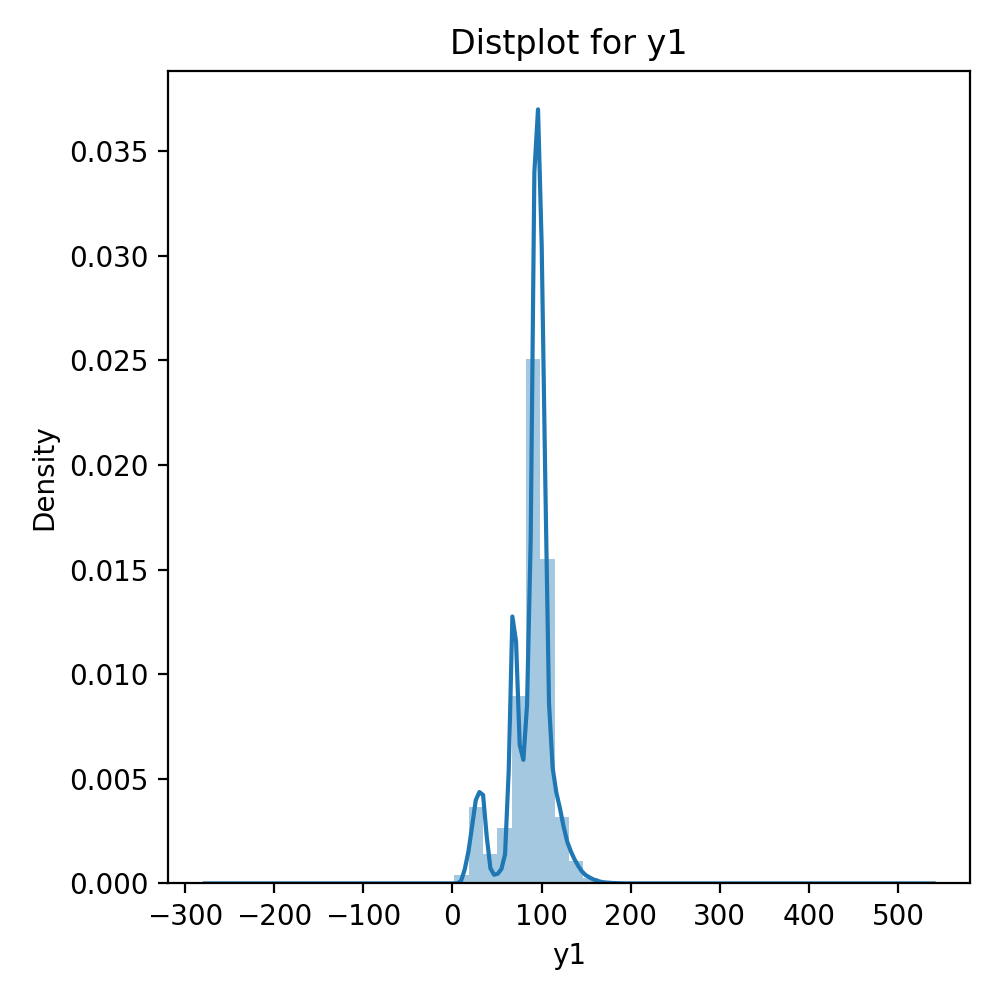
\includegraphics[width=1\linewidth]{y1prescaling}
        \caption{Distribuzione di y1 prima del min-max-scaling.}
        \label{fig:distprescaling:y1}
    \end{subfigure}
    %
    \\
    \begin{subfigure}[t]{0.4\textwidth}
        \centering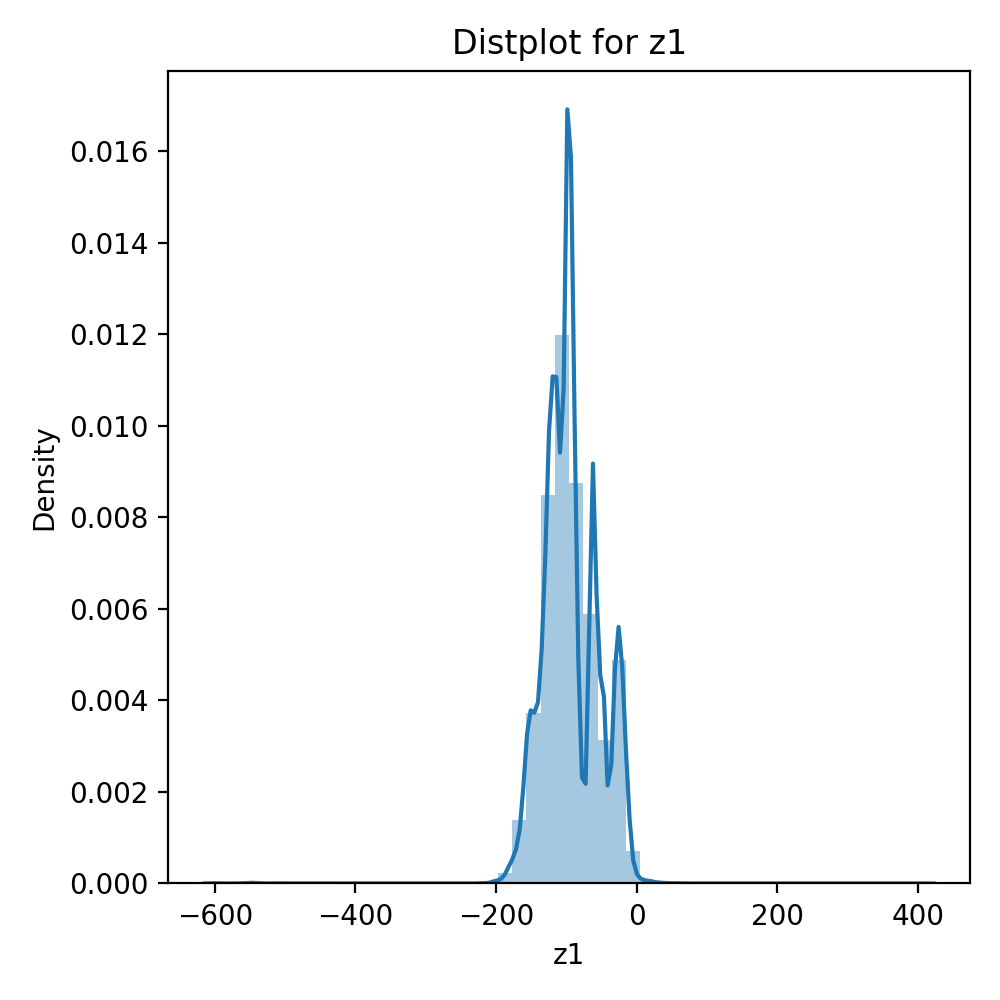
\includegraphics[width=1\linewidth]{z1prescaling}
        \caption{Distribuzione di z1 prima del min-max-scaling.}
        \label{fig:distprescaling:z1}
    \end{subfigure}
    %
    \begin{subfigure}[t]{0.4\textwidth}
        \centering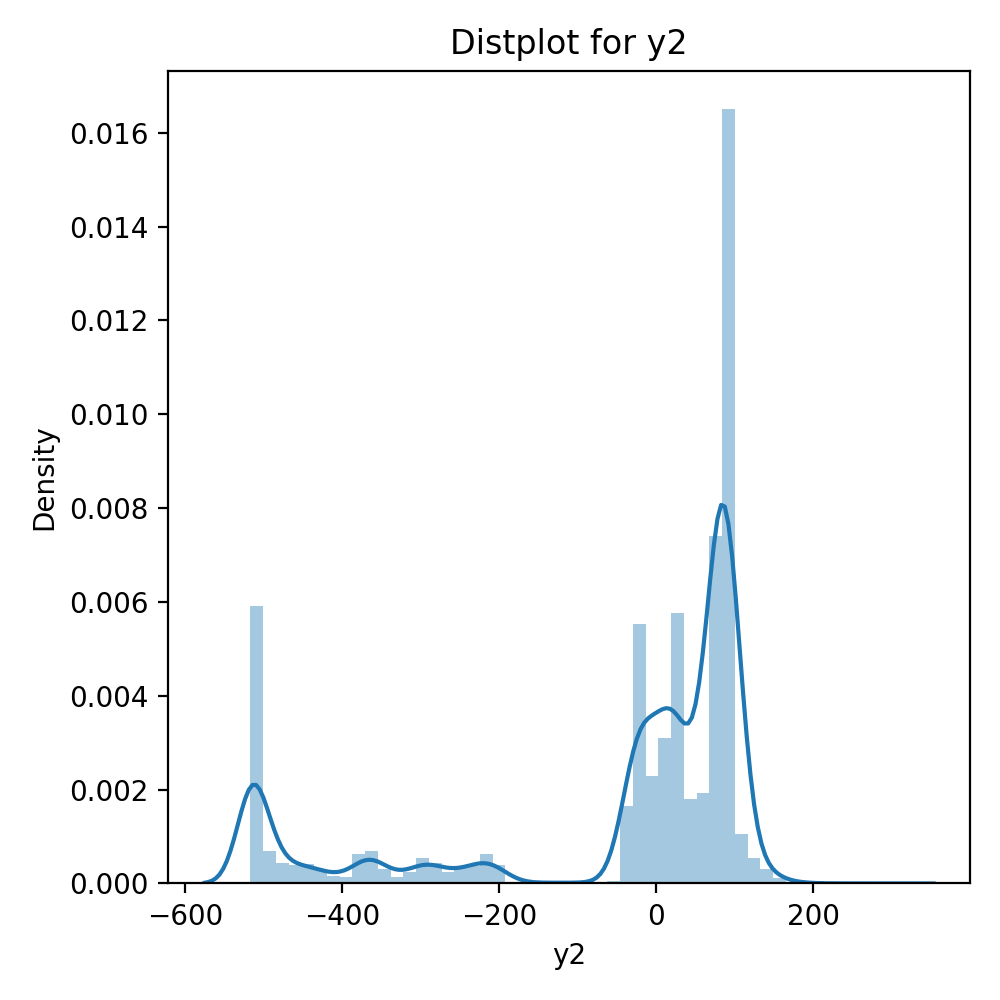
\includegraphics[width=1\linewidth]{y2prescaling}
        \caption{Distribuzione di y2 prima del min-max-scaling.}
        \label{fig:distprescaling:y2}
    \end{subfigure}
    \caption{Distribuzione di variabili prima del min-max-scaling.}
    \label{fig:distprescaling}
\end{figure}

In figura \ref{fig:distprescaling} sono mostrati i grafici di distribuzione di alcune variabili prima di aver subito il min-max-scaling, come si vede i valori variano nell'ordine delle centinaia intorno allo zero.

\begin{figure}[ht]
    \centering
    \begin{subfigure}[t]{0.4\textwidth}
        \centering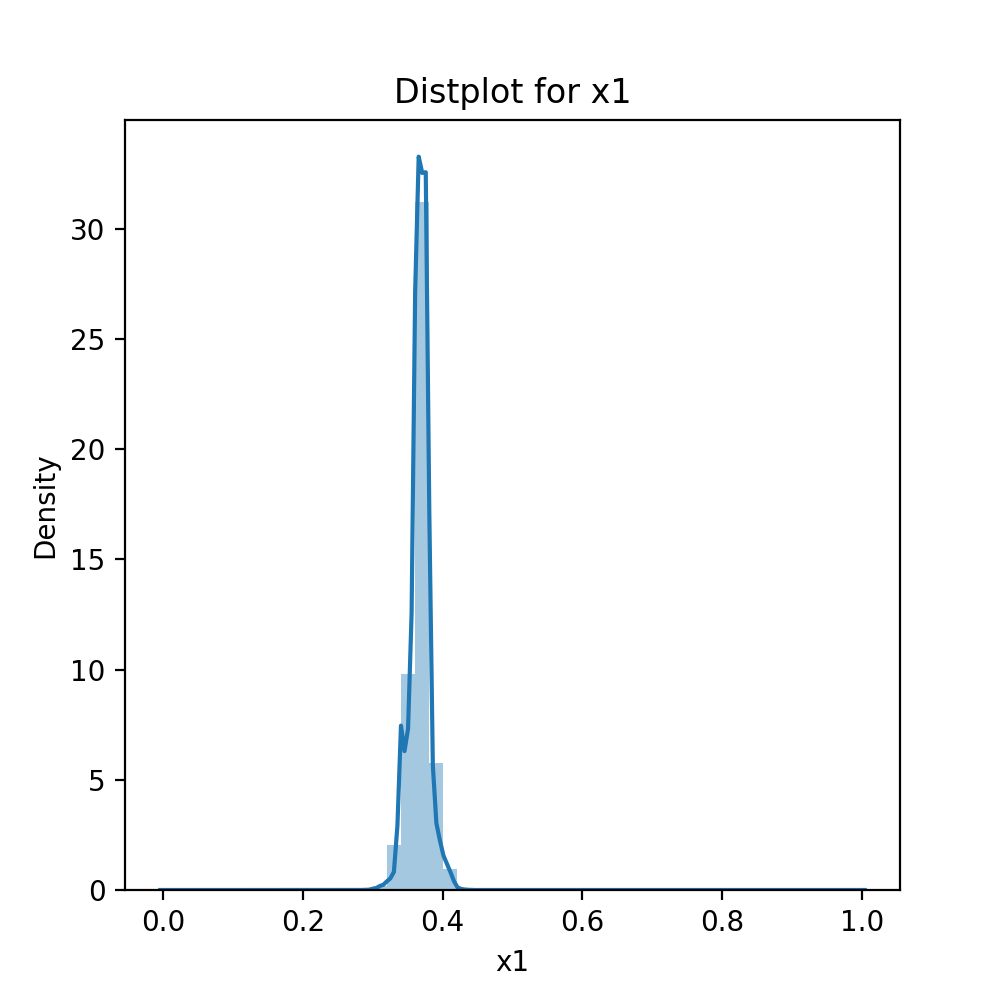
\includegraphics[width=1\linewidth]{x1postscaling}
        \caption{Distribuzione di x1 dopo il min-max-scaling.}
        \label{fig:distpostscaling:x1}
    \end{subfigure}
    %
    \begin{subfigure}[t]{0.4\textwidth}
        \centering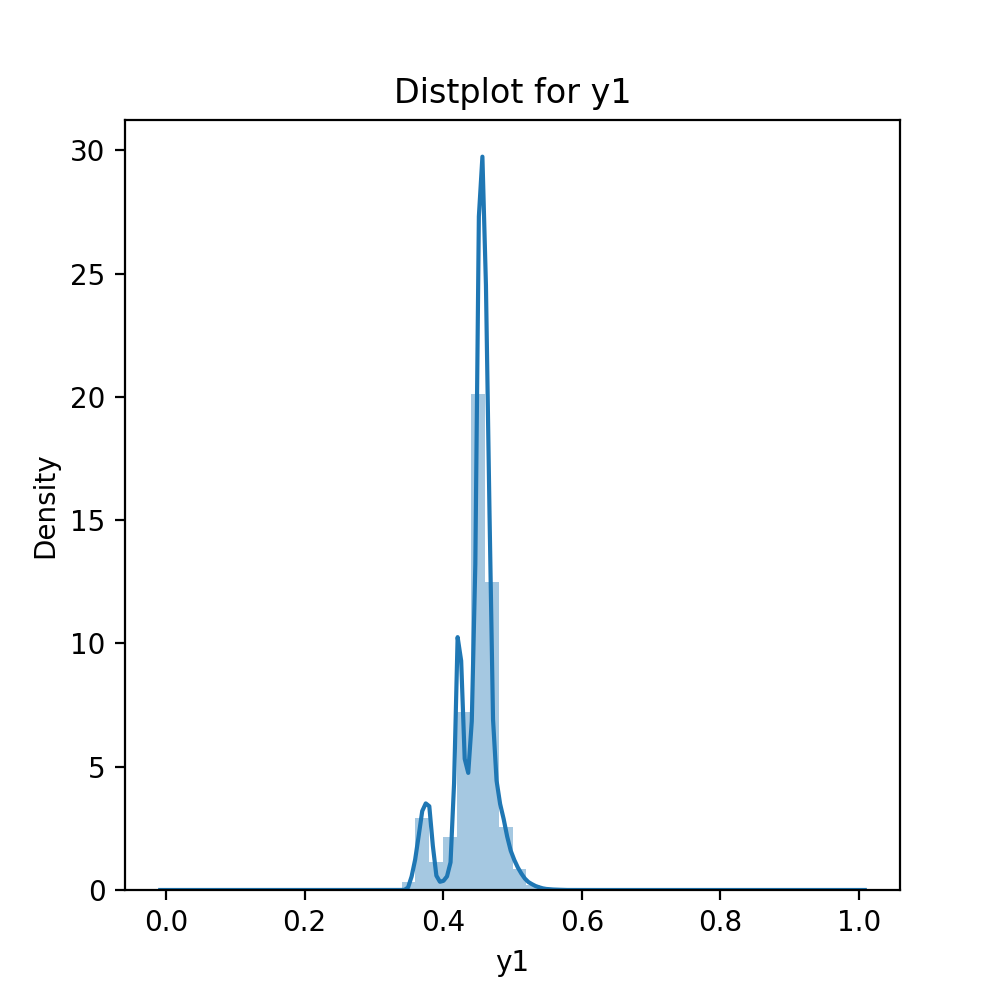
\includegraphics[width=1\linewidth]{y1postscaling}
        \caption{Distribuzione di y1 dopo il min-max-scaling.}
        \label{fig:distpostscaling:y1}
    \end{subfigure}
    %
    \\
    \begin{subfigure}[t]{0.4\textwidth}
        \centering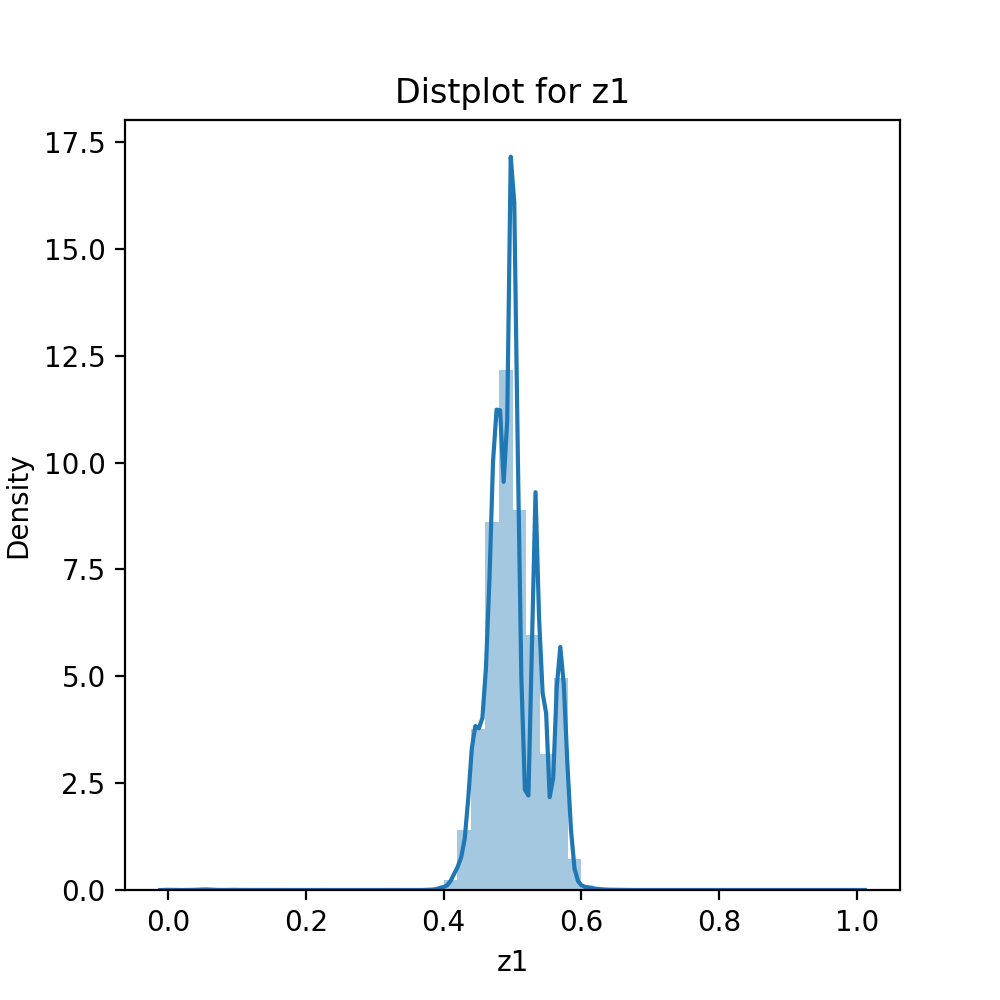
\includegraphics[width=1\linewidth]{z1postscaling}
        \caption{Distribuzione di z1 dopo il min-max-scaling.}
        \label{fig:distpostscaling:z1}
    \end{subfigure}
    %
    \begin{subfigure}[t]{0.4\textwidth}
        \centering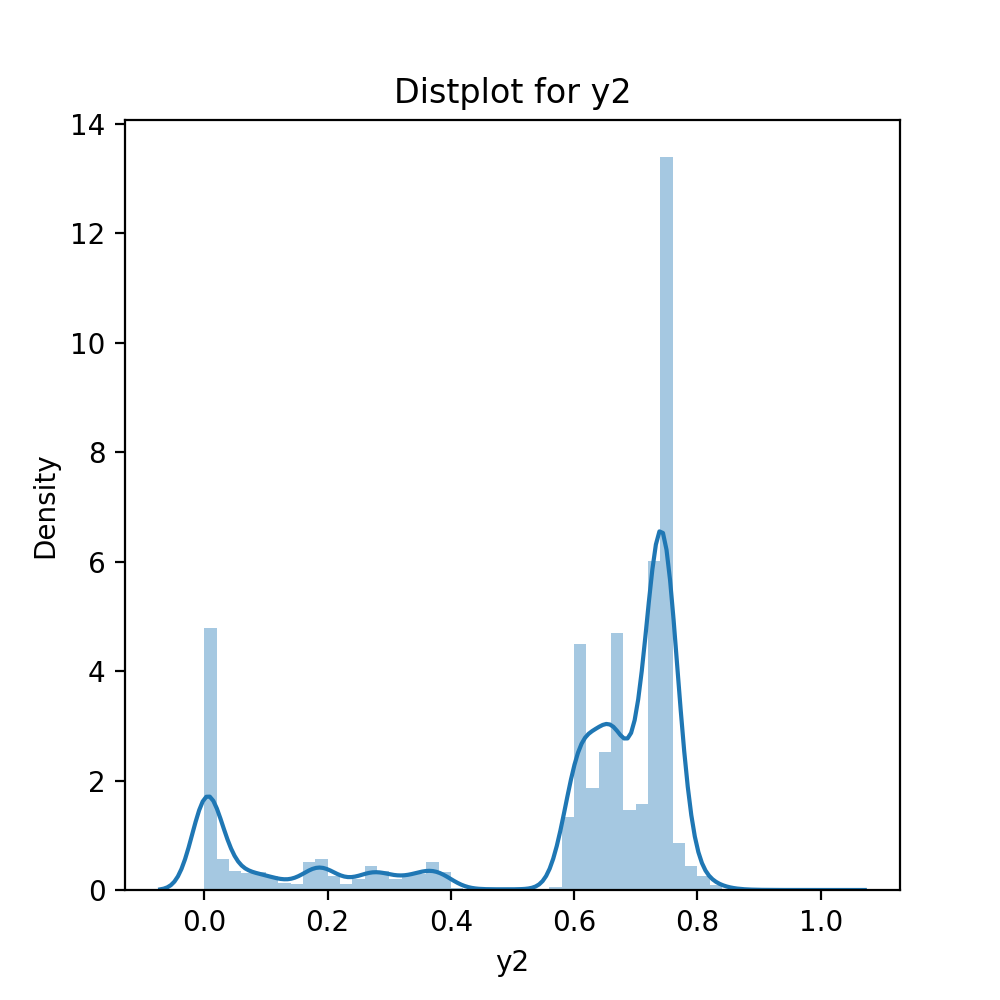
\includegraphics[width=1\linewidth]{y2postscaling}
        \caption{Distribuzione di y2 dopo il min-max-scaling.}
        \label{fig:distpostscaling:y2}
    \end{subfigure}
    \caption{Distribuzione di variabili dopo il min-max-scaling.}
    \label{fig:distpostscaling}
\end{figure}

In figura \ref{fig:distpostscaling} invece sono mostrati i grafici delle distribuzioni delle stesse variabili dopo aver subito la trasformazione del min-max-scaling, come si vede il valore è compreso tra 0 e 1 ma l'andamento è lo stesso e la distribuzione mantiene la stessa forma, a prova del fatto che i dati mantengono le stesse informazioni rappresentative. Grazie a quest'operazione di trasformazione delle features i modelli saranno più efficienti e veloci in fase di training.

Infine per due dei tre modelli testati è stata fatta un'ulteriore operazione di riduzione delle features, infatti per le seconde e terze versioni dei modelli \textit{SVM} e \textit{rete neurale} è stata applicata la \textbf{principal component analysis} (PCA), un metodo che riduce il numero delle features proiettando i punti in un sottospazio più piccolo dimensionalmente rispetto allo spazio originario delle features. Il modello decision tree è più efficiente in termini di prestazioni e velocità, quindi non è stato applicato il metodo PCA a questo algoritmo perché già efficiente con le features selezionate precedentemente. Le SVM e le reti neurali invece essendo più lente nella fase di training sono state velocizzate dalla riduzione delle features fatta dalla PCA. 

Per ogni variante del modello è stata fatta una selezione degli iperparametri tramite cross-validation per model selection, per valutare quali iperparametri portano ad un modello migliore, dopodiché è stata applicata la cross-validation per model assessment, cioè per stimare le prestazioni che avrà il modello ricavato dalla model selection. La model selection è stata effettuata usando l'oggetto \verb+GridSearchCV+ di \textit{scikit-learn} \cite{sklearn}, in particolare applica la strategia di cross-validation \textbf{K-fold}: il training set viene diviso in K parti uguali, K-1 parti vengono usate come training set mentre la parte rimanente viene usata come validation set, questo processo viene ripetuto K volte cambiando ogni volta la parte del validation set, infine le prestazioni del modello vengono calcolate come media delle prestazioni nelle K iterazioni. Il parametro K è stato mantenuto quello di default, cioè K = 5. Per la fase di model assessment è stata utilizzata la funzione di \textit{scikit-learn} \cite{sklearn} \verb+cross_validate()+, che divide il dataset passato come parametro in training set e development set, addestra il modello, passato anch'esso come parametro, sul training set e ne valuta le prestazione sul development set in base a certe metriche specificate. In questo caso la valutazione è stata fatta con le metriche \textbf{F1-score} e \textbf{accuracy bilanciata}.

\subsection{Decision Tree}
\subsubsection{Prima versione}\label{subsubsec:dtv1}
Per la prima versione dell'algoritmo \textit{Decision tree} è stata fatta la model selection testando i seguenti iperparametri:
\begin{itemize}
\item \textbf{max\_depth}: rappresenta la profondità massima che l'albero decisionale può avere, sono stati testati i valori \textit{5, 10, 20, 50}.
\item \textbf{class\_weight}: è il peso da dare a ogni classe, i valori testati sono \textit{balanced} che assegna un peso a ogni classe sulla base del bilanciamento che questa classe ha nel dataset di riferimento, e il valore \textit{None} che assegna un peso uguale a ogni classe.
\item \textbf{criterion}: l'indicatore con cui misurare l'impurità dei nodi, i valori testati sono \textit{gini} che usa l'indice di Gini per l'impurità, e il valore \textit{entropy} che utilizza una seconda metodologia per calcolare l'impurità.
\item \textbf{splitter}: la strategia con cui dividere i nodi, cioè il valore su cui fare il test per ogni nodo, sono stati testati i valori \textit{best}, cioè scegliendo lo splitting migliore, e il valore \textit{random} con il quale invece lo splitting viene scelto casualmente.
\end{itemize}

Dopo la fase di model selection sono stati ricavati i migliori valori per ogni iperparametro, rappresentati in tabella \ref{tab:dtv1}, che portano ad avere un valore di F1-score, usata per la cross-validation, pari a 0.985.

\begin{table}[h] 
\centering
\begin{tabular}{l l}
\hline
\textbf{max\_depth} & \textit{20}\\
\textbf{class\_weight} & \textit{None}\\
\textbf{criterion} & \textit{entropy}\\
\textbf{splitter} & \textit{best}\\
\hline
\end{tabular}
\caption{Iperparametri migliori per la prima versione del Decision tree.}
\label{tab:dtv1}
\end{table}

Con la fase di model assessment si sono ricavate le metriche: $$F1-score = 0.985$$ $$accuracy\_bilanciata = 0.974$$

Inoltre per l'algoritmo Decision tree è possibile analizzare l'importanza di ogni features per valutare quali features sono più incisive sulla classificazione, in figura \ref{fig:featuresimportancedtv1} è mostrata la features importance per la prima versione del modello Decision tree, dalla quale si nota che le tre features più importanti sono le coordinate \textit{z1}, \textit{z2} e \textit{y3}, probabilmente queste tre variabili influiscono molto sul riconoscimento della postura rispetto alle altre variabili con importanza minore. 

\begin{figure}[h]
    \centering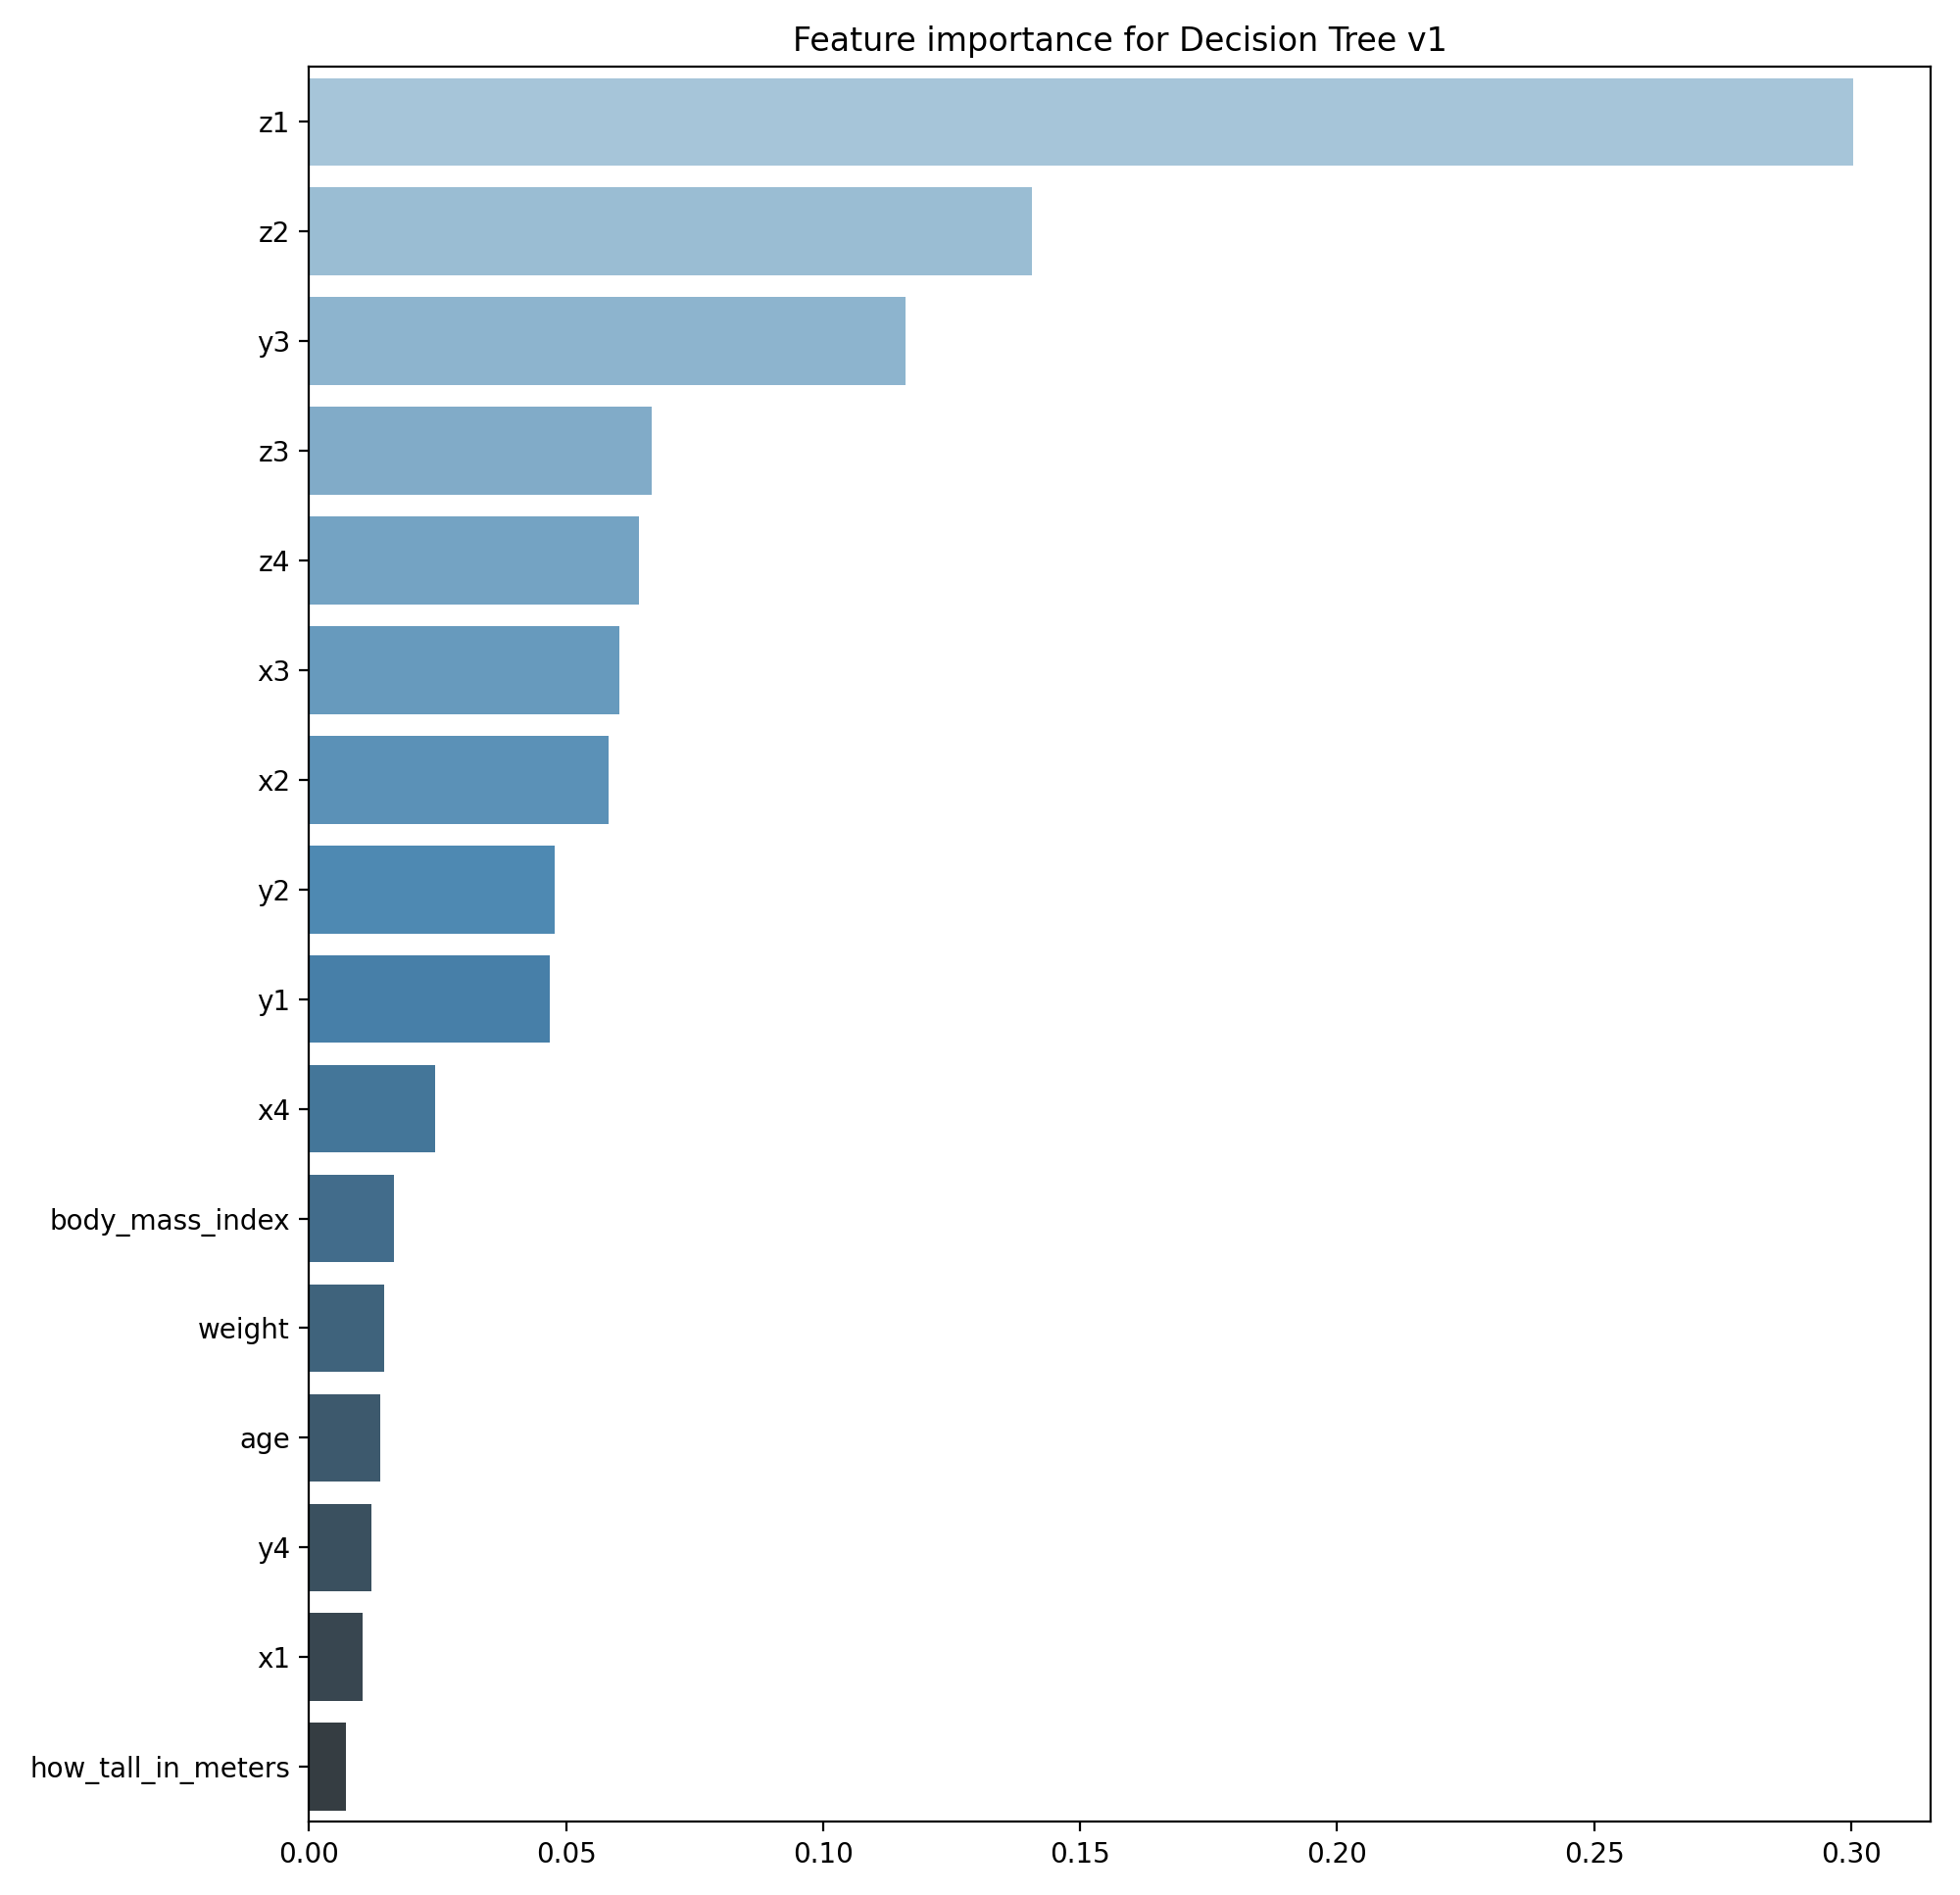
\includegraphics[width=0.6\linewidth]{featimportdtv1}
    \caption{Features importance per la prima versione del modello Decision tree.}
    \label{fig:featuresimportancedtv1}
\end{figure}

\subsubsection{Seconda versione}
Per la seconda versione vengono utilizzati i dati pre-processati come descritto nella sezione \ref{subsec:prepr}.  Gli iperparametri testati durante la model selection sono gli stessi testati per la prima versione del decsion tree (si veda \ref{subsubsec:dtv1}), con i valori rappresentati in tabella \ref{tab:valdtv2}, mentre in tabella \ref{tab:dtv2} sono mostrati i valori migliori ricavati dopo la model selection, che portano ad un valore ottimo di F1-score pari a 0.980, in questo caso quindi c'è un leggero degrado delle prestazioni.

\begin{table}[h] 
\centering
\begin{tabular}{l l}
\hline
\textbf{max\_depth} & \textit{5, 10, 20, 50}\\
\textbf{class\_weight} & \textit{balanced, None}\\
\textbf{criterion} & \textit{gini, enotrpy}\\
\textbf{splitter} & \textit{best, random}\\
\hline
\end{tabular}
\caption{Valori testati per gli iperparametri della seconda versione del Decision tree.}
\label{tab:valdtv2}
\end{table}

\begin{table}[h] 
\centering
\begin{tabular}{l l}
\hline
\textbf{max\_depth} & \textit{50}\\
\textbf{class\_weight} & \textit{None}\\
\textbf{criterion} & \textit{enotrpy}\\
\textbf{splitter} & \textit{best}\\
\hline
\end{tabular}
\caption{Iperparametri migliori per la seconda versione del Decision tree.}
\label{tab:dtv2}
\end{table}

Con la fase di model assessment, per la seconda versione del Decision tree, le metriche ricavate sono:
$$F1-score = 0.980$$
$$accuracy\_bilanciata = 0.967$$

Anche la metrica \textit{accuracy\_bilanciata} quindi mostra un degrado delle prestazioni rispetto alla prima versione.
Infine anche per questa seconda versione si analizza l'importanza delle features, mostrata in figura \ref{fig:featuresimportancedtv2}, dalla quale si nota che le variabili \textit{z1} e \textit{y3} rimangono molto importanti come nella prima versione, in questo caso però la variabile \textit{z2} essendo stata eliminata nella fase di features selection non è presente, e assume molta importanza la variabile \textit{y2}.

\begin{figure}[h]
    \centering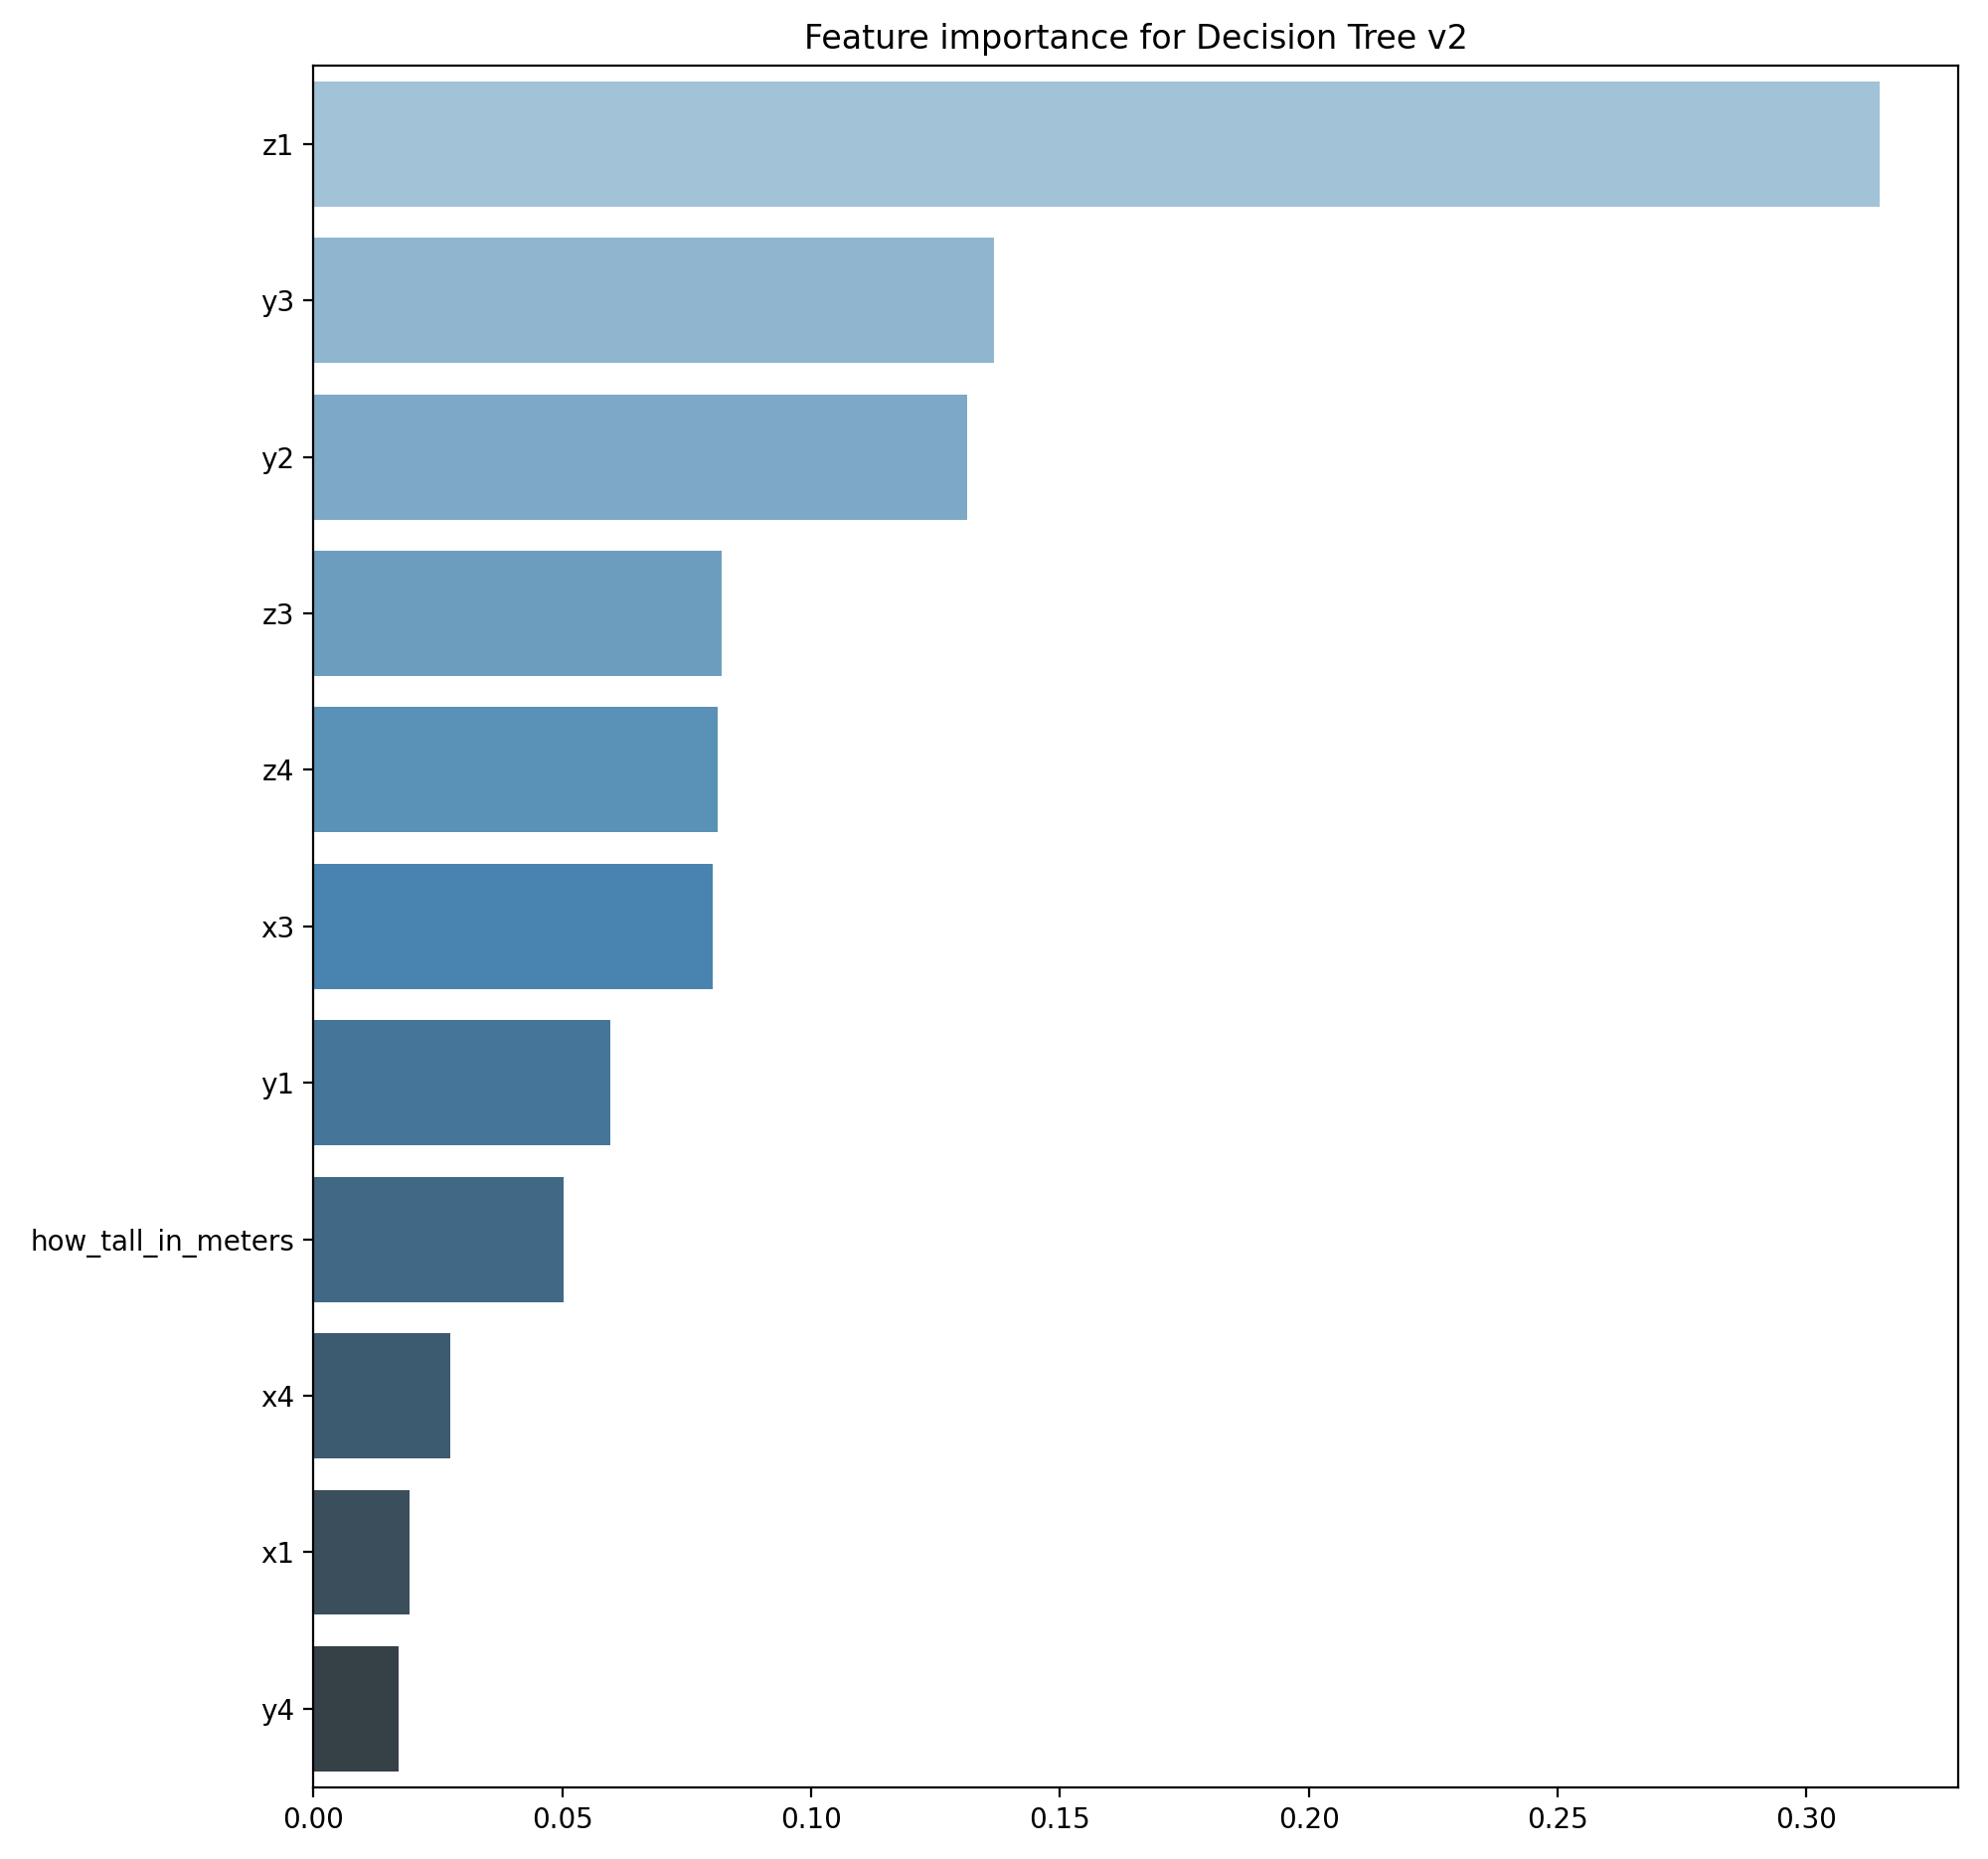
\includegraphics[width=0.6\linewidth]{featimportdtv2}
    \caption{Features importance per la seconda versione del modello Decision tree.}
    \label{fig:featuresimportancedtv2}
\end{figure}

\subsubsection{Terza versione}
La terza versione è costituita da un modello in ensemble della migliore tra le prime due varianti, in questo caso come visto dalle metriche la versione che garantisce una migliore classificazione è la prima, di conseguenza verrà usata questa per creare il modello in ensemble, e come training set sarà quindi mantenuto quello della prima versione, senza pre-processing.

L'algoritmo sarà costruito usando il metodo del \textit{RandomForest}, che rappresenta appunto una versione ensemble del Decision tree, cioè addestrerà tanti Decision tree e unirà le loro predizioni per ottenere un risultato migliore di quello che raggiungerebbe un singolo decision tree. I valori degli iperparametri in questo caso saranno gli stessi di quelli trovati con la model selection nella prima versione, mentre la model selection per questa versione sarà fatta esclusivamente sull'iperparametro \textbf{n\_estimators}, che rappresenta il numero di decision tree che il modello in ensemble dovrà addestrare., in particolare i valori testati sono \textit{5, 10, 20, 50}. In tabella \ref{tab:dtv3} vediamo quindi i valori ottimi degli iperaparametri di questa versione, che portano a un valore ottimo di F1-score = 0.995.

\begin{table}[h] 
\centering
\begin{tabular}{l l}
\hline
\textbf{max\_depth} & \textit{20}\\
\textbf{class\_weight} & \textit{None}\\
\textbf{criterion} & \textit{enotrpy}\\
\textbf{n\_estimators} & \textit{50}\\
\hline
\end{tabular}
\caption{Iperparametri migliori per la terza versione del Decision tree.}
\label{tab:dtv3}
\end{table}

Durante la fase di model assessment sono stati ricavati i valori delle metriche di valutazione:
$$F1-score = 0.995$$
$$accuracy\_bilanciata = 0.992$$

La variante in ensemble garantisce quindi un discreto incremento di prestazioni rispetto a entrambe le versioni precedenti. In figura \ref{fig:featuresimportancedtv3} è mostrata l'importanza delle features per questa terza versione.

\begin{figure}[h]
    \centering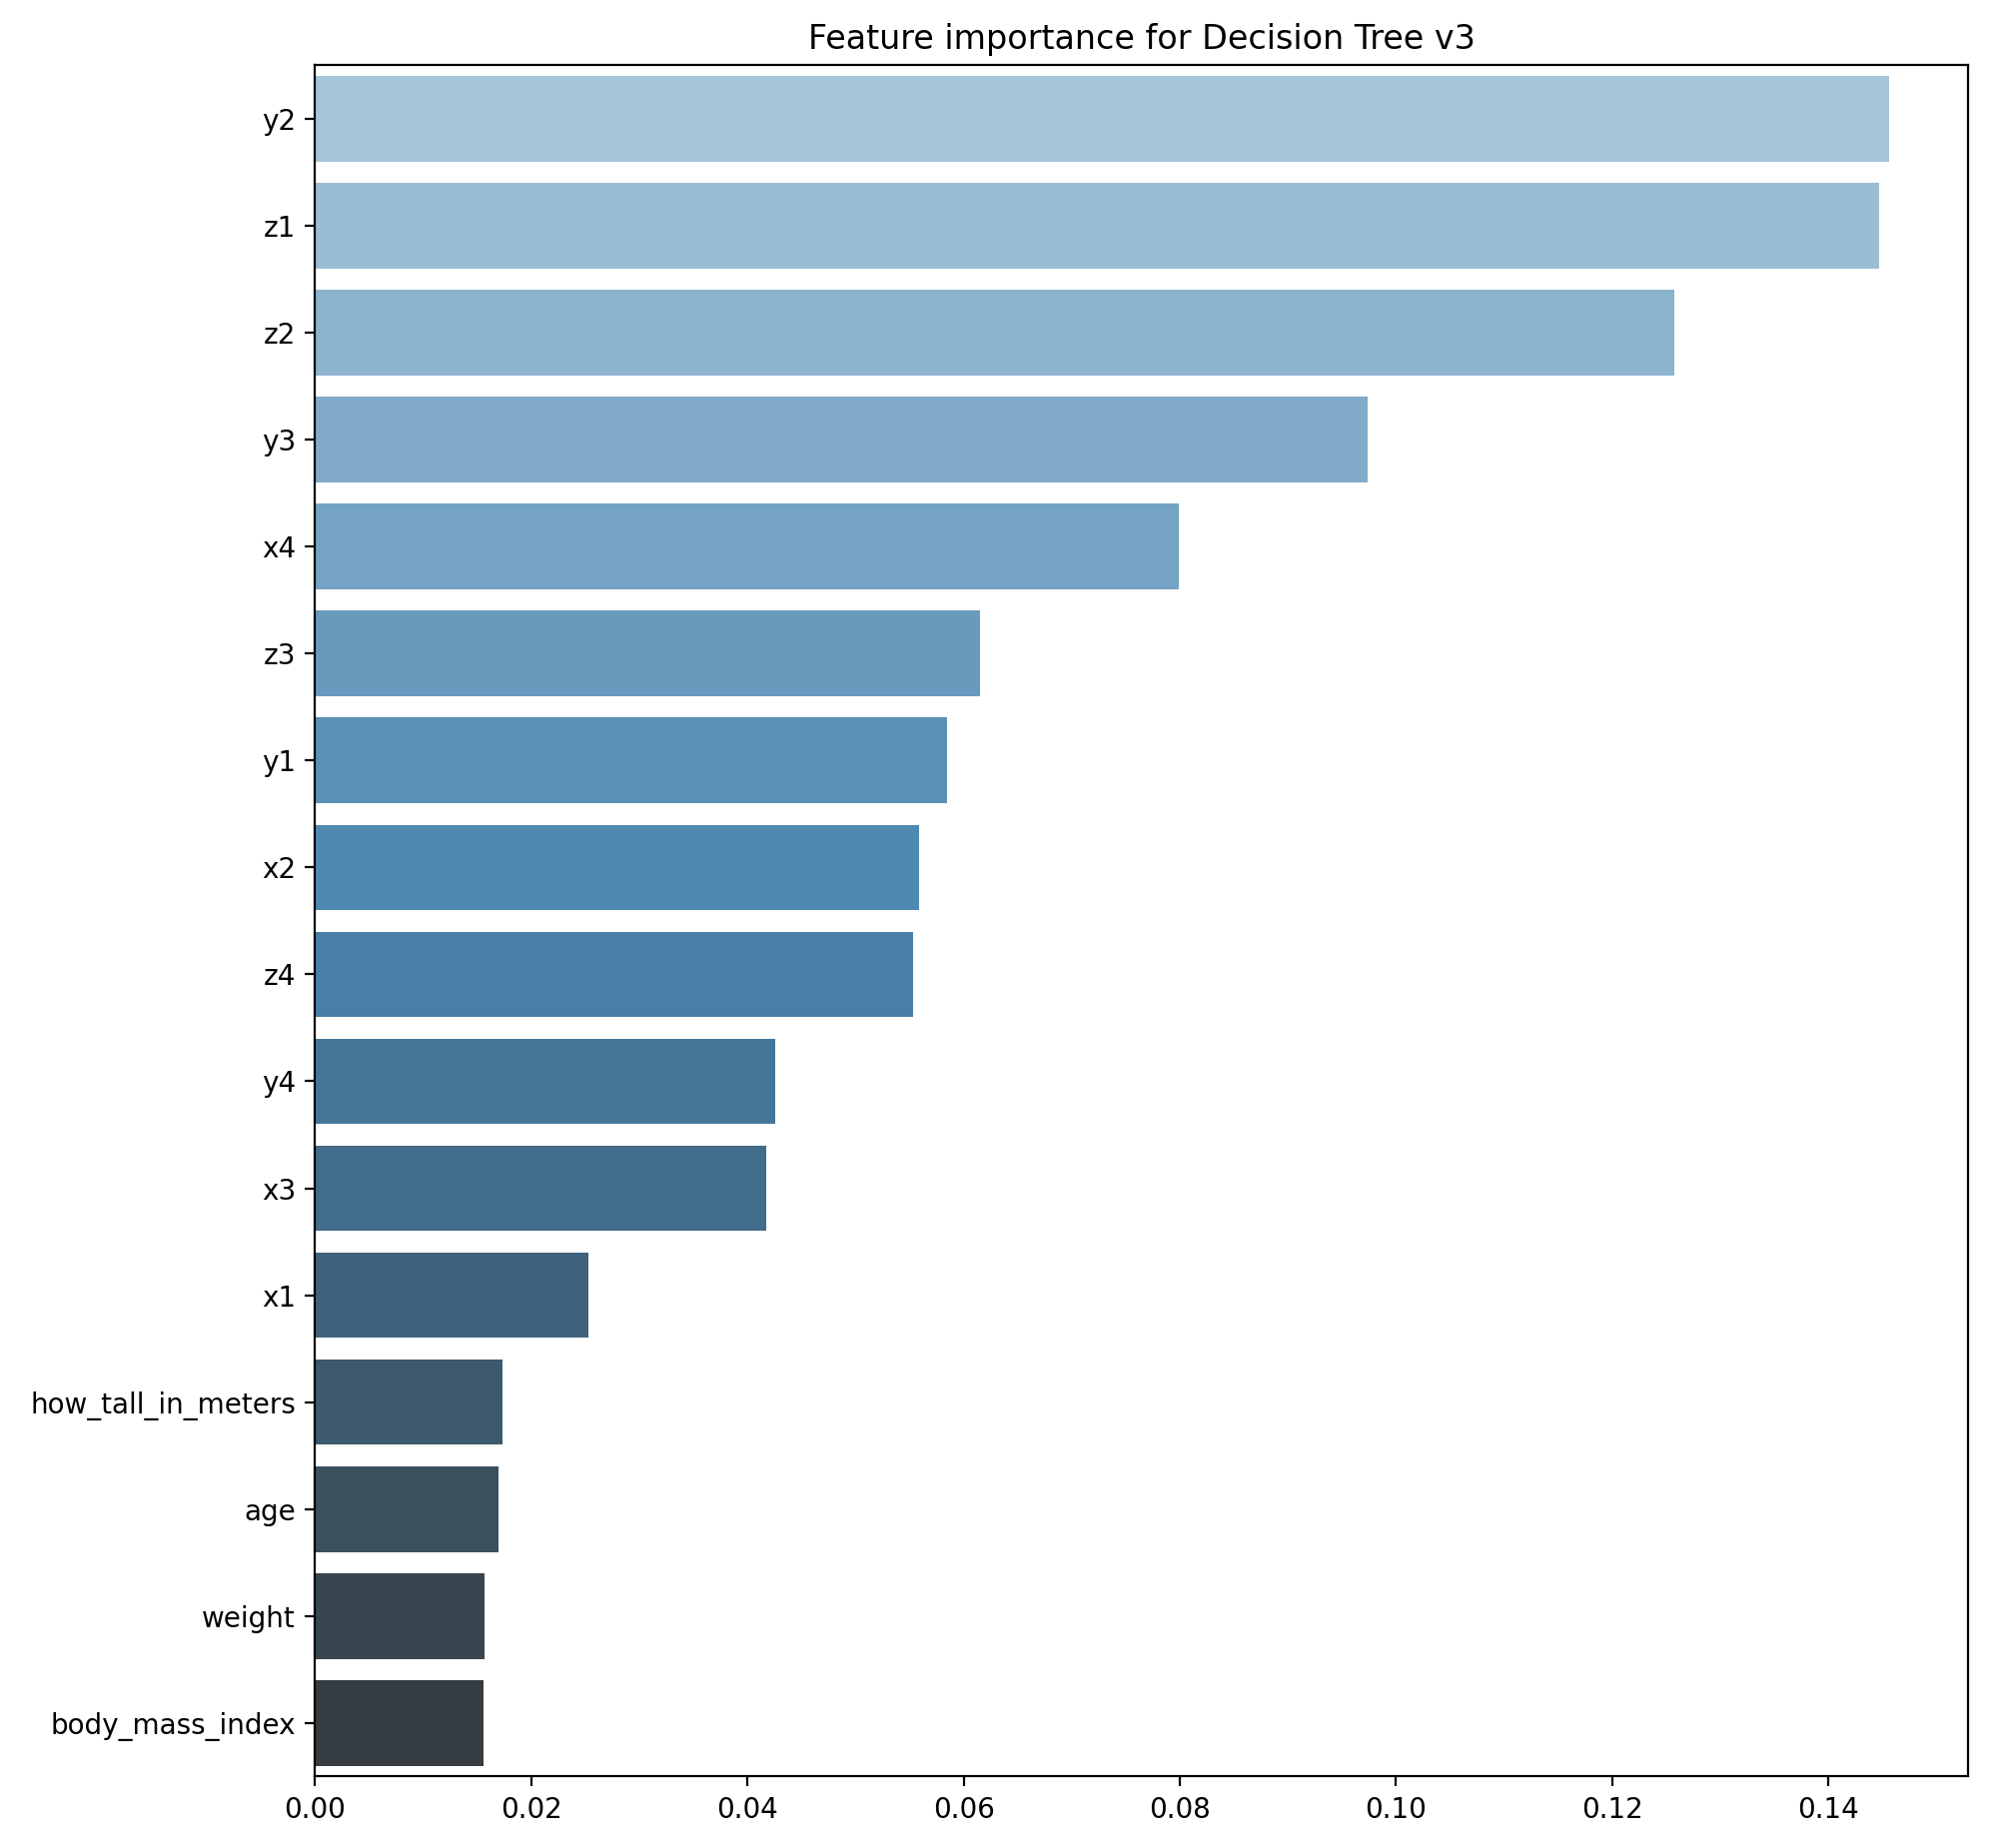
\includegraphics[width=0.6\linewidth]{featimportdtv3}
    \caption{Features importance per la terza verisone del modello Decision tree.}
    \label{fig:featuresimportancedtv3}
\end{figure}

\subsection{Support Vector Machine}
\subsubsection{Prima versione}\label{subsubsec:svmv1}
Per la prima versione del modello \textit{SVM}, durante la model selection, sono stati testati i seguenti iperparametri:
\begin{itemize}
\item \textbf{C}: è il coefficiente di regolarizzazione che regola il trade-off tra grandezza del margine ed errori commessi dall'algoritmo, i valori testati sono \textit{0.1 e 1000}.
\item \textbf{kernel}: rappresenta la funzione usata come kernel trick, cioè per mappare le features in uno spazio dimensionalmente diverso, i valori testati sono \textit{linear}, cioè la funzione lineare, \textit{poly} per avere una funzione polinomiale, e \textit{rbf} per usare la radial basis function.
\item \textbf{class\_weight}: come bilanciare le classi, sono stati testati i valori \textit{balanced} per bilanciare le classi nel modo in cui sono bilanciare nel dataset, e \textit{None} per assegnare lo stesso peso a tutte le classi.
\item \textbf{max\_iter}: il numero massimo di iterazioni che l'algoritmo può fare, i valori testati sono \textit{10, 50}.
\item \textbf{decision\_function\_shape}: è la metodologia con cui adattare il modello binario per un problema multiclasse, i valori testati sono \textit{ovo}, cioè lo \textit{One-vs-One}, e \textit{ovr}, cioò lo \textit{One-vs-Rest}.
\end{itemize}

Con la fase di model selection sono stati ricavati i valori migliori per ogni iperaparametro, mostrati in tabella \ref{tab:svmv1}, che portano a un valore di F1-score = 0.468.

\begin{table}[h] 
\centering
\begin{tabular}{l l}
\hline
\textbf{C} & \textit{1000}\\
\textbf{kernel} & \textit{rbf}\\
\textbf{class\_weight} & \textit{balanced}\\
\textbf{max\_iter} & \textit{10}\\
\textbf{decision\_function\_shape} & \textit{ovo}\\
\hline
\end{tabular}
\caption{Iperparametri migliori per la prima versione di SVM.}
\label{tab:svmv1}
\end{table}

Il model assessment garantisce le prestazioni seguenti:
$$F1-score = 0.468$$
$$accuracy\_bilanciata = 0.423$$

\subsubsection{Seconda versione}\label{subsubsec:svmv2}
La seconda versione della \textit{SVM} utilizza i dati pre-processati e inoltre utilizza la \textit{PCA} tramite una \textit{pipeline}, un modo che mette in sequenza una metodologia di trasformazione dei dati, in questo caso la PCA, e un modello di learning, la SVM. La fase di model selection testerà tutti gli iperparametri testati per la prima versione \ref{subsubsec:svmv1} per quanto riguarda la SVM, inoltre testerà anche il parametro \textit{n\_components}, cioè il numero di componenti della PCA. I valori testati per questo iperparametro sono \textit{1, 5, 10, 20}.
I valori ottimi risultanti sono mostrati in tabella \ref{tab:svmv2} e sono relativi a un valore di F1-score = 0.555.

\begin{table}[h] 
\centering
\begin{tabular}{l l}
\hline
\textbf{C} & \textit{1000}\\
\textbf{kernel} & \textit{rbf}\\
\textbf{class\_weight} & \textit{None}\\
\textbf{max\_iter} & \textit{50}\\
\textbf{decision\_function\_shape} & \textit{ovo}\\
\textbf{n\_components} & \textit{10}\\
\hline
\end{tabular}
\caption{Iperparametri seconda versione SVM.}
\label{tab:svmv2}
\end{table}

In questo caso si ottengono delle prestazioni leggermente superiori rispetto alla prima versione,  seppur non ancora soddisfacenti, infatti i valori delle metriche ottenute dal model assessment sono:
$$F1-score = 0.567$$
$$accuracy\_bilanciata = 0.530$$

\subsubsection{Terza versione}\label{subsubsec:svmv3}
L'algoritmo della terza versione sarà una versione ensemble della seconda versione, in quanto la migliore tra le prime due, di conseguenza il training set usato sarà quello delle seconde versioni, cioè quello con il pre-processing. È stata utilizzata la tecnica di ensemble detta \textbf{Bagging}: si addestrano tanti \textit{weak learner} parallelamente e in modo indipendente e si unisce il risultato di ognuno in modo deterministico. In particolare è stato usato l'oggetto \verb+BaggingClassifier+ di \textit{scikit-learn} \cite{sklearn}, il quale prende un modello di base e ne addestra un certo numero, ognuno su un sottoinsieme diverso del dataset originario, infine ne combina i vari risultati in un risultato unico. Il parametro \textit{base\_estimator} sarà il modello SVM della seconda versione, che sarà il modello base su cui il classificatore di ensemble si baserà. Durante la model selection sarà valutato solamente il parametro \textit{n\_estimators} che rappresenta il numero di weak learner da addestrare, i valori testati per questo iperparametro sono \textit{10, 50, 100}. Il valore ottimo ottenuto dalla fase di model selection è 100, e porta ad avere un'F1-score pari a 0.615. Infine la fase di model assessment restituisce le metriche:
$$F1-score = 0.610$$
$$accuracy\_bilanciata = 0.602$$

Quindi la tecnica di ensemble migliora le prestazioni del modello originale, aumentando sia la F1-score che l'accuracy bilanciata, nonostante ciò la bontà di questo modello non eccelle e i valori rimangono piuttosto bassi.

\subsection{Reti neurali}
\subsubsection{Prima versione}\label{nnv1}
Gli iperparametri testati durante la cross-validation per la prima versione delle reti neurali sono i seguenti:
\begin{itemize}
\item \textbf{hidden\_layer\_sizes}: rappresenta il numero di layer che la rete avrà e quanti nodi ogni layer avrà, viene rappresentato sotto forma di \textit{tupla} Python, dove ogni elemento rappresenta un layer e il numero stesso rappresenta il numero di nodi di quel layer. I valori testati sono \textit{(50, 50), (20, 20, 20), (5, 5, 5, 5)}.
\item \textbf{max\_iter}: è il numero massimo di iterazioni che l'algoritmo farà, i valori testati sono \textit{10, 50}.
\item \textbf{early\_stopping}: parametro che indica se adottare o no l'early stopping per evitare l'overfitting, in questo si testano i valori \textit{True, False}.
\item \textbf{activation}: è la funzione di attivazione dei nodi della rete, sono stati testati i valori \textit{logistic}, che rappresenta la funzione sigmoide, e il valore \textit{tanh}, che rappresenta la funzione tangente iperbolica.
\end{itemize}

In tabella \ref{tab:nnv1} sono rappresentati i valori ottimi per ciascun iperparametro trovati con la model selection, che portano ad un valore dell'F1-score uguale a 0.980.

\begin{table}[h] 
\centering
\begin{tabular}{l l}
\hline
\textbf{hidden\_layer\_sizes} & \textit{(50, 50)}\\
\textbf{max\_iter} & \textit{50}\\
\textbf{early\_stopping} & \textit{False}\\
\textbf{max\_iter} & \textit{50}\\
\textbf{activation} & \textit{logistic}\\
\hline
\end{tabular}
\caption{Iperparametri migliori per la prima versione della rete neurale.}
\label{tab:nnv1}
\end{table}

Dalla fase di model assessment si ricavano i valori:
$$F1-score = 0.980$$
$$accuracy\_bilanciata = 0.965$$

\subsubsection{Seconda versione}\label{nnv2}
Per la seconda versione della rete neurale si utilizzano i dati pre-processati e la PCA, nello stesso modo in cui è utilizzata nella seconda versione della SVM (si veda \ref{subsubsec:svmv2}), cioè usando la pipeline tra la PCA e il modello vero e proprio.  Gli iperparametri testati durante la model selection sono gli stessi testati nella prima versione della rete neurale e descritti nella sezione \ref{nnv1} e in più il parametro \textit{n\_components} della PCA, testato con i valori \textit{1, 5, 10, 20}. I valori ottimi ottenuti in questo caso sono mostrati nella tabella \ref{tab:nnv2} e portano ad avere una F1-score = 0.990.

\begin{table}[h] 
\centering
\begin{tabular}{l l}
\hline
\textbf{hidden\_layer\_sizes} & \textit{(50, 50)}\\
\textbf{max\_iter} & \textit{50}\\
\textbf{early\_stopping} & \textit{False}\\
\textbf{max\_iter} & \textit{50}\\
\textbf{activation} & \textit{tanh}\\
\textbf{n\_components} & \textit{10}\\
\hline
\end{tabular}
\caption{Iperparametri migliori della seconda versione della rete neurale.}
\label{tab:nnv2}
\end{table}

La model assessment mostra i valori delle metriche:
$$F1-score = 0.990$$
$$accuracy\_bilanciata = 0.985$$
La seconda versione ha quindi un miglioramento dal punto di vista delle prestazioni e risulta più precisa.

\subsubsection{Terza versione}\label{nnv3}
La terza variante della rete neurale sarà una versione ensemble della seconda versione, dato che quest'ultima è la migliore. Saranno quindi usati i dati pre-processati come training set. Il metodo di ensemble utilizzato in questo caso è lo stesso descritto nella sezione \ref{subsubsec:svmv3}, cioè si usa il \textit{BaggingClassifier} che avrà come modello di base la pipeline relativa alla seconda versione della rete neurale, e verrà fatta la valutazione del solo parametro \textit{n\_estimators} con i valori \textit{10, 20, 50}, che avrà come valore ottimo 20, con un valore di F1-score stimato pari a 0.989.

Infine il processo di model assessment garantisce i valori:
$$F1-score = 0.992$$
$$accuracy\_bilanciata = 0.986$$
Rispetto alla versione due quindi si ha un leggero aumento delle prestazioni grazie alla metodologia di ensemble.

\subsection{Metriche di valutazione}
Per valutare le prestazioni complessive del modello, dopo le fasi di cross-validation per model selection e model assessment, l'algoritmo viene riaddestrato sull'intero training set iniziale, quello senza pre-processing per le prime versioni e quello pre-processato per le seconde e terze versioni, e infine testato sul test set, di cui è stato fatto lo splitting al 20\% all'inizio e mai toccato prima di questa fase finale di testing. La valutazione è stata fatta usando le seguenti metriche:
\begin{itemize}
\item \textbf{Accuracy bilanciata}, perché come visto nella sezione \ref{sec:analisi} il dataset iniziale è sbilanciato rispetto alla variabile target, quindi è necessario usare un bilanciamento;
\item \textbf{Precision}, calcolata come la percentuale di predizioni corrette di una certa classe sul totale delle predizioni con quella label. Essendo un problema multiclasse il valore finale è calcolato come media pesata dei vari valori delle classi;
\item \textbf{Recall}, calcolata come la percentuale di predizioni corrette di una certa classe rispetto al totale di samples effettivamente appartenenti a quella classe. Anche in questo il valore finale è calcolato come media pesata dei valori delle varie classi;
\item \textbf{F1-score}, calcolata come
\begin{equation}
F1-score = \frac{2 \times Precision \times Recall}{Precision+Recall}
\end{equation}
\end{itemize}

L'analisi delle prestazioni complessive dei vari modelli e dei risultati finali è approfondita nella prossima sezione \ref{sec:risultati}.